\newpage
\section{Durchführung}
\label{sec:Durchführung}

\subsection{Versuchsaufbau}
\label{subsec:Versuchsaufbau}

Der Versuchsaufbau besteht aus einer Röntgenröhre mit einer Kupfer Anode einem
$LiF$ -Kristall und einem Geiger-Müller-Zählrohr. Die Elektronik der Apparatur kann
mithilfe eines Computers gesteuert werden. Über das Messprogramm können außerdem die
Daten direkt aufgenommen und abgespeichert werden, sowie die Messbereiche eingestellt
werden.
\begin{figure}[H]
  \centering
  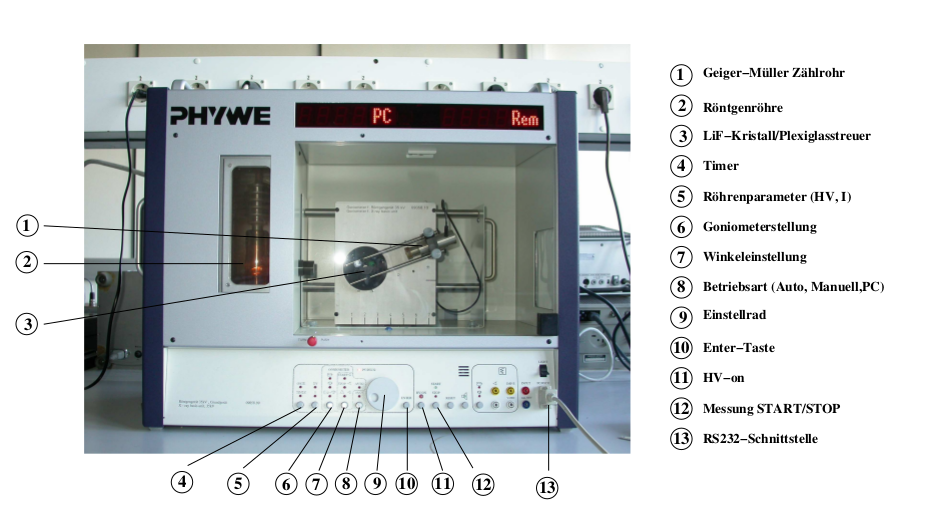
\includegraphics[width=16.6cm,height=9.8cm]{Aufbau.png}
  \caption{Aufbau der im Versuch benutzten Röntgen-Röhre \cite{sample}.}
  \label{fig:Aufbau}
\end{figure}
Für die Messungen wird eine Beschleunigungsspannung $U_\symup{B} = \SI{35}{\kilo\volt}$ und ein
Emissionsstrom von $I = \SI{1}{\milli\ampere}$ angelegt. Außerdem wird die allgemeine Funktionalität
der Eletronik und der Messaperatur festgestellt.\\

\subsection{Durchführung der Messreihen}
\label{subsec:Messreihen}

Es werden insgesamt drei unterschiedliche Messreihen durchgeführt. \\
Bei der erste Messung wird die Braggbedingung überprüft, das heißt es wird ein fester
Kristallwinkel bei $\Theta_\symup{LiF} = \SI{14}{\degree}$ eingestellt und dann mit dem
Geiger-Müller-Zählrohr in dem Bereich $ \SI{26}{\degree} \leq \alpha_\symup{GM} \leq
\SI{30}{\degree}$, mit der Schrittgröße $\symup{\Delta} \alpha = \SI{0.1}{\degree}$, die
Intensität der Röntgenstrahlung gemessen.\\
\newpage
Die zweite Messreihe ist eine Messung des Röntgenspektrum. Dabei wird der sogenannte
\enquote{$2 \colon \!\! 1$ Kopplungsmodus} eingestellt, das heißt für jeden Winkelschritt
den der Kristall sich dreht, dreht sich das Geiger-Müller-Zählrohr um doppelt so viel.
Es wird in dem Bereich $\SI{4}{\degree} \leq \Theta \leq \SI{26}{\degree}$ gemessen
mit einer Schrittgöße von $\symup{\Delta} \alpha = \SI{0.2}{\degree}$ und einer
Integrationszeit von $\symup{\Delta} t = \SI{5}{\second}$.\\
Für die letzte Messreihe werden vier Messungen durchgeführt, jede davon mit einem anderen
Absorber vor dem Geiger-Müller-Zählrohr. Es wird dabei jeweils in einem geeigneten
Intervall, welches im Bereich um den Braggwinkel der $K$ und $L$-Linen liegt,
gemessen. Wird mit einer Schrittgöße von $\symup{\Delta} \alpha
= \SI{0.1}{\degree}$ und einer Integrationszeit von $\symup{\Delta} t = \SI{20}{\second}$
gearbeitet.
